% Alex header 
\documentclass[aps,amsmath,amssymb,amsfont]{scrartcl}
\usepackage[utf8]{inputenc}
\usepackage[T1]{fontenc}
%\usepackage[german]{babel}
\usepackage{float}
\usepackage{graphicx}
%\usepackage{siunitx}
\usepackage[colorlinks=true,linkcolor=black]{hyperref}
\usepackage{lmodern}
\usepackage{mathpazo}
\usepackage{here}
\usepackage{amsmath}
\usepackage{mathtools}
\usepackage[utf8]{inputenc}
\usepackage[T1]{fontenc}
\usepackage{subcaption}
\usepackage{placeins}
\usepackage{braket}
\numberwithin{equation}{section}
\usepackage{tikz}
\usetikzlibrary{arrows, calc, decorations.pathmorphing}
\tikzset{snake/.style={decorate, decoration=snake}}
\usepackage[europeanresistors,americaninductors]{circuitikz}
\makeatletter
\AtBeginDocument{
\def\tocname{Content}
	\def\andname{and}
	\def\Dated@name{Dated: }
	\def\figurename{Fig.}
	\def\tablename{Tab.}
}
\makeatother

\definecolor{grey}{rgb}{0.5,0.5,0.5}

\newcommand{\subfig}[1]{\begin{subfigure}[t]{0.49\textwidth}
        \centering
        \includegraphics[width=1.1\textwidth]{#1}
        \caption{}	
    \end{subfigure}}
\newcommand{\pictures}[1]{\begin{subfigure}[t]{0.49\textwidth}
        \centering
        \includegraphics[width=1.1\textwidth]{#1}
        \caption{}
    \end{subfigure}}


%Michael header
%\documentclass[
%    captions=nooneline
%    ,headinclude
%    ,headsepline
%    ,bibliography=totocnumbered
%]{scrartcl}
%\usepackage[twoside,paper=a4paper,left=35mm,right=20mm,top=30mm,bottom=35mm]{geometry} 

%\usepackage[T1]{fontenc}
%\usepackage[utf8]{inputenc}
\usepackage[german]{varioref}

%%% GRAPHIKEN %%%
%\usepackage{graphicx}
\usepackage[labelfont=bf,justification=justified,format=plain]{caption}
\usepackage{subcaption}
\usepackage{placeins}
\usepackage{wrapfig}
%\graphicspath{{../Photonenstatistik_Messdaten/}}
%\usepackage{floatrow}
%% DREHUNG VON GRAFIKEN
%\usepackage{rotating}
%\usepackage{pdflscape}

%%% Tabellen %%%
%\usepackage{threeparttable}
%\usepackage{booktabs}
%\usepackage{multirow}
\usepackage{longtable}

%%% MATHE %%%
%\usepackage{mathtools}
%\usepackage{physics}
%\usepackage{upgreek}
%\usepackage{amssymb}
\usepackage[separate-uncertainty=true,
            list-units = single,
            list-separator = {;\,},
            exponent-product=\cdot,%
            ]{siunitx}
%\DeclareSIUnit\molar{\mole\per\l}
%\DeclareSIUnit\counts{counts}

%%% ZEICHENUMGEBUNG %%%
\usepackage{pgf}


%%% BIBLIOGRAPHIE %%%
\usepackage[style=numeric-comp,backend=biber,natbib=true]{biblatex}
\addbibresource{Quellen.bib}
\usepackage[babel,german]{csquotes}

%%% EIGENE DEFINITIONEN %%%
%\newcommand{\iu}{{i\mkern1mu}}
%\usepackage{txfonts} % |R, |C

%\usepackage{hyperref}

%%% INCLUDE VALUES %%%
%\newcommand{\bigtableplus}{
\begin{tabular}{S[table-format=+3.1]S[table-format=+2]|S[table-format=3]S[table-format=3]S[table-format=3]S[table-format=3]S[table-format=3]}
{$\alpha$ [\si{\degree}]}&{$\beta$ [\si{\degree}]}&\multicolumn{5}{c}{$C(\alpha,\beta)$ [counts/s]}\\\hline
22.5&0&170&172&166&165&161\\
22.5&90&624&627&616&622&606\\
112.5&0&644&648&632&639&627\\
112.5&90&176&177&179&178&173\\\hline
22.5&-45&158&157&145&151&154\\
22.5&45&628&632&656&641&631\\
112.5&-45&646&665&661&652&680\\
112.5&45&131&149&145&150&151\\\hline
-22.5&0&145&141&141&153&141\\
-22.5&90&599&593&592&577&593\\
67.5&0&640&623&637&623&634\\
67.5&90&123&121&120&127&121\\\hline
-22.5&-45&636&642&642&642&649\\
-22.5&45&166&171&168&174&183\\
67.5&-45&196&210&201&211&203\\
67.5&45&558&563&562&562&549\\\hline
\end{tabular}}

\newcommand{\bigtableminus}{
\begin{tabular}{S[table-format=+3.1]S[table-format=+2]|S[table-format=3]S[table-format=3]S[table-format=3]S[table-format=3]S[table-format=3]}
{$\alpha$ [\si{\degree}]}&{$\beta$ [\si{\degree}]}&\multicolumn{5}{c}{$C(\alpha,\beta)$ [counts/s]}\\\hline
22.5&0&84&91&89&84&88\\
22.5&90&634&629&630&624&615\\
112.5&0&625&618&622&624&625\\
112.5&90&79&73&76&80&75\\\hline
22.5&-45&441&448&453&450&448\\
22.5&45&267&265&260&264&272\\
112.5&-45&274&269&280&264&268\\
112.5&45&407&423&415&421&430\\\hline
-22.5&0&248&258&252&254&247\\
-22.5&90&448&459&441&450&444\\
67.5&0&535&514&502&503&514\\
67.5&90&218&211&213&215&219\\\hline
-22.5&-45&94&97&96&102&96\\
-22.5&45&616&627&607&630&611\\
67.5&-45&647&637&632&621&631\\
67.5&45&108&103&107&109&111\\\hline
\end{tabular}}

\newcommand{\bigtabletom}{
\begin{tabular}{S[table-format=2]|ll|S[table-format=+2]S[table-format=+2]|S[table-format=2]S[table-format=2]||S[table-format=3]S[table-format=3]S[table-format=3]S[table-format=3]S[table-format=3]}
&{S1}&{S2}&{P1 [\si{\degree}]}&{L1 [\si{\degree}]}&{P2 [\si{\degree}]}&{L2 [\si{\degree}]}&\multicolumn{5}{c}{$C(\alpha,\beta)$ [counts/s]}\\\hline
1&$\state{H}$&$\state{H}$&0&0&0&0&49&48&52&48&49\\
2&$\state{H}$&$\state{V}$&0&0&90&0&647&647&647&641&647\\
3&$\state{V}$&$\state{V}$&90&0&90&0&49&47&43&45&47\\
4&$\state{V}$&$\state{H}$&90&0&0&0&683&669&660&665&686\\
5&$\state{R}$&$\state{H}$&90&45&0&0&413&396&402&409&409\\
6&$\state{R}$&$\state{V}$&90&40&90&0&300&283&297&292&293\\
7&$\state{D}$&$\state{V}$&45&45&90&0&419&434&426&420&416\\
8&$\state{D}$&$\state{H}$&45&45&0&0&303&307&312&308&303\\
9&$\state{D}$&$\state{R}$&45&45&45&0&399&391&388&392&378\\
10&$\state{D}$&$\state{D}$&45&45&45&45&621&622&628&628&618\\
11&$\state{R}$&$\state{D}$&45&0&45&45&382&378&385&378&392\\
12&$\state{H}$&$\state{D}$&0&0&45&45&259&267&268&269&270\\
13&$\state{V}$&$\state{D}$&90&0&45&45&436&422&435&425&428\\
14&$\state{V}$&$\state{L}$&90&0&0&45&351&342&345&338&344\\
15&$\state{H}$&$\state{L}$&0&0&0&45&394&385&401&387&396\\
16&$\state{R}$&$\state{L}$&0&-45&0&45&55&54&50&55&48\\
\hline
\end{tabular}}

\newcommand{\Ma}{
\frac{1}{2}\begin{pmatrix}
2&1&-1+i&-1-i\\
1&0&0&0\\
-1-i&0&0&i\\
-1+i&0&-i&0
\end{pmatrix}}

\newcommand{\Mb}{
\frac{1}{2}\begin{pmatrix}
0&1&-1+i&0\\
1&0&-1+i&0\\
-1-i&-1-i&2&i\\
0&0&-i&0
\end{pmatrix}}

\newcommand{\Mc}{
\frac{1}{2}\begin{pmatrix}
0&1&0&0\\
1&2&-1+i&-1-i\\
0&-1-i&0&i\\
0&-1+i&-i&0
\end{pmatrix}}

\newcommand{\Md}{
\frac{1}{2}\begin{pmatrix}
0&1&0&-1-i\\
1&0&0&-1-i\\
0&0&0&i\\
-1+i&-1+i&-i&2
\end{pmatrix}}

\newcommand{\Me}{
\frac{1}{2}\begin{pmatrix}
0&-1-i&0&2i\\
-1+i&0&0&0\\
0&0&0&-1-i\\
-2i&0&1+i&0
\end{pmatrix}}

\newcommand{\Mf}{
\frac{1}{2}\begin{pmatrix}
0&-1-i&0&0\\
-1+i&0&-2i&0\\
0&2i&0&1-i\\
0&0&1+i&0
\end{pmatrix}}

\newcommand{\Mg}{
\frac{1}{2}\begin{pmatrix}
0&-1-i&0&0\\
-1+i&0&2&0\\
0&2&0&-1+i\\
0&0&-1-i&0
\end{pmatrix}}

\newcommand{\Mh}{
\frac{1}{2}\begin{pmatrix}
0&-1-i&0&2\\
-1+i&0&0&0\\
0&0&0&-1+i\\
2&0&-1-i&0
\end{pmatrix}}

\newcommand{\Mi}{
\frac{1}{2}\begin{pmatrix}
0&2i&0&0\\
-2i&0&0&0\\
0&0&0&-2i\\
0&0&2i&0
\end{pmatrix}}

\newcommand{\Mj}{
\frac{1}{2}\begin{pmatrix}
0&2&0&0\\
2&0&0&0\\
0&0&0&2\\
0&0&2&0
\end{pmatrix}}

\newcommand{\Mk}{
\frac{1}{2}\begin{pmatrix}
0&2i&0&0\\
-2i&0&0&0\\
0&0&0&2i\\
0&0&-2i&0
\end{pmatrix}}

\newcommand{\Ml}{
\frac{1}{2}\begin{pmatrix}
0&-1-i&2&0\\
-1+i&0&0&0\\
2&0&0&-1-i\\
0&0&-1+i&0
\end{pmatrix}}

\newcommand{\Mm}{
\frac{1}{2}\begin{pmatrix}
0&-1-i&0&0\\
-1+i&0&0&2\\
0&0&0&-1-i\\
0&2&-1+i&0
\end{pmatrix}}

\newcommand{\Mn}{
\frac{1}{2}\begin{pmatrix}
0&-1+i&0&0\\
-1-i&0&0&2i\\
0&0&0&1-i\\
0&-2i&1+i&0
\end{pmatrix}}

\newcommand{\Mo}{
\frac{1}{2}\begin{pmatrix}
0&-1+i&-2i&0\\
-1-i&0&0&0\\
2i&0&0&1-i\\
0&0&1+i&0
\end{pmatrix}}

\newcommand{\Mp}{
\frac{1}{2}\begin{pmatrix}
0&2&0&0\\
2&0&0&0\\
0&0&0&-2\\
0&0&-2&0
\end{pmatrix}}

\newcommand{\rhonormal}{
\begin{pmatrix}
0.035+0.000i &-0.034+0.056i &-0.057-0.032i &-0.038+0.032i\\
-0.034-0.056i &0.033+0.000i &0.054+0.037i &0.049-0.011i\\
-0.057+0.032i &0.054-0.037i &0.457+0.000i &0.120-0.000i\\
-0.038-0.032i &0.049+0.011i &0.407+0.000i &0.476+0.000i
\end{pmatrix}}

\newcommand{\drhonormal}{
\begin{pmatrix}
0.001+0.000i &0.025+0.024i &0.005+0.006i &0.007+0.009i\\
0.025+0.024i &0.002+0.000i &0.007+0.006i &0.009+0.007i\\
0.005+0.006i &0.007+0.006i &0.007+0.000i &0.021+0.029i\\
0.007+0.009i &0.009+0.007i &0.024+0.029i &0.013+0.000i
\end{pmatrix}}

\newcommand{\evala}{0.706}\newcommand{\eveca}{
\begin{pmatrix}
-0.098+0.028i\\
0.110+0.018i\\
0.467-0.022i\\
0.871+0.000i
\end{pmatrix}}

\newcommand{\evalb}{0.259}\newcommand{\evecb}{
\begin{pmatrix}
0.027+0.209i\\
0.092-0.145i\\
-0.472+0.073i\\
0.835+0.000i
\end{pmatrix}}

\newcommand{\evalc}{-0.036}\newcommand{\evecc}{
\begin{pmatrix}
0.719+0.000i\\
0.264+0.627i\\
-0.005-0.112i\\
0.046+0.068i
\end{pmatrix}}

\newcommand{\evald}{0.071}\newcommand{\evecd}{
\begin{pmatrix}
0.687+0.000i\\
-0.195-0.606i\\
0.237-0.058i\\
-0.160+0.195i
\end{pmatrix}}

\newcommand{\rhobell}{
\begin{pmatrix}
0.000+0.000i &0.001-0.056i &0.004+0.013i &-0.007-0.008i\\
0.001+0.056i &0.067+0.000i &-0.100-0.013i &-0.012-0.056i\\
0.004-0.013i &-0.100+0.013i &0.730+0.000i &0.134+0.000i\\
-0.007+0.008i &-0.012+0.056i &-0.153-0.000i &0.202+0.000i
\end{pmatrix}}

\newcommand{\drhobell}{
\begin{pmatrix}
0.027+0.024i &0.027+0.024i &0.014+0.014i &0.014+0.014i\\
0.027+0.024i &0.027+0.024i &0.014+0.014i &0.014+0.014i\\
0.014+0.014i &0.014+0.014i &0.032+0.029i &0.032+0.029i\\
0.014+0.014i &0.014+0.014i &0.032+0.029i &0.032+0.029i
\end{pmatrix}}



%\includeonly{}

%\tikzset{
%    declare function={% in case of CVS which switches the arguments of atan2
%        atan3(\a,\b)=ifthenelse(atan2(0,1)==90, atan2(\a,\b), atan2(\b,\a));},
%    kinky cross radius/.initial=+.125cm,
%    @kinky cross/.initial=+, kinky crosses/.is choice,
%    kinky crosses/left/.style={@kinky cross=-},kinky crosses/right/.style={@kinky cross=+},
%    kinky cross/.style args={(#1)--(#2)}{
%        to path={
%            let \p{@kc@}=($(\tikztotarget)-(\tikztostart)$),
%            \n{@kc@}={atan3(\p{@kc@})+180} in
%            -- ($(intersection of \tikztostart--{\tikztotarget} and #1--#2)!%
%            \pgfkeysvalueof{/tikz/kinky cross radius}!(\tikztostart)$)
%            arc [ radius     =\pgfkeysvalueof{/tikz/kinky cross radius},
%            start angle=\n{@kc@},
%            delta angle=\pgfkeysvalueof{/tikz/@kinky cross}180 ]
%%            -- (\tikztotarget)}}}

\usepackage{physics}

% Own commands
\newcommand{\state}[1]{\left|\text{#1}\right\rangle}
\newcommand{\brastate}[1]{\left\langle\text{#1}\right|}


\newcommand{\bigtableplus}{
\begin{tabular}{S[table-format=+3.1]S[table-format=+2]|S[table-format=3]S[table-format=3]S[table-format=3]S[table-format=3]S[table-format=3]}
{$\alpha$ [\si{\degree}]}&{$\beta$ [\si{\degree}]}&\multicolumn{5}{c}{$C(\alpha,\beta)$ [counts/s]}\\\hline
22.5&0&170&172&166&165&161\\
22.5&90&624&627&616&622&606\\
112.5&0&644&648&632&639&627\\
112.5&90&176&177&179&178&173\\\hline
22.5&-45&158&157&145&151&154\\
22.5&45&628&632&656&641&631\\
112.5&-45&646&665&661&652&680\\
112.5&45&131&149&145&150&151\\\hline
-22.5&0&145&141&141&153&141\\
-22.5&90&599&593&592&577&593\\
67.5&0&640&623&637&623&634\\
67.5&90&123&121&120&127&121\\\hline
-22.5&-45&636&642&642&642&649\\
-22.5&45&166&171&168&174&183\\
67.5&-45&196&210&201&211&203\\
67.5&45&558&563&562&562&549\\\hline
\end{tabular}}

\newcommand{\bigtableminus}{
\begin{tabular}{S[table-format=+3.1]S[table-format=+2]|S[table-format=3]S[table-format=3]S[table-format=3]S[table-format=3]S[table-format=3]}
{$\alpha$ [\si{\degree}]}&{$\beta$ [\si{\degree}]}&\multicolumn{5}{c}{$C(\alpha,\beta)$ [counts/s]}\\\hline
22.5&0&84&91&89&84&88\\
22.5&90&634&629&630&624&615\\
112.5&0&625&618&622&624&625\\
112.5&90&79&73&76&80&75\\\hline
22.5&-45&441&448&453&450&448\\
22.5&45&267&265&260&264&272\\
112.5&-45&274&269&280&264&268\\
112.5&45&407&423&415&421&430\\\hline
-22.5&0&248&258&252&254&247\\
-22.5&90&448&459&441&450&444\\
67.5&0&535&514&502&503&514\\
67.5&90&218&211&213&215&219\\\hline
-22.5&-45&94&97&96&102&96\\
-22.5&45&616&627&607&630&611\\
67.5&-45&647&637&632&621&631\\
67.5&45&108&103&107&109&111\\\hline
\end{tabular}}

\newcommand{\bigtabletom}{
\begin{tabular}{S[table-format=2]|ll|S[table-format=+2]S[table-format=+2]|S[table-format=2]S[table-format=2]||S[table-format=3]S[table-format=3]S[table-format=3]S[table-format=3]S[table-format=3]}
&{S1}&{S2}&{P1 [\si{\degree}]}&{L1 [\si{\degree}]}&{P2 [\si{\degree}]}&{L2 [\si{\degree}]}&\multicolumn{5}{c}{$C(\alpha,\beta)$ [counts/s]}\\\hline
1&$\state{H}$&$\state{H}$&0&0&0&0&49&48&52&48&49\\
2&$\state{H}$&$\state{V}$&0&0&90&0&647&647&647&641&647\\
3&$\state{V}$&$\state{V}$&90&0&90&0&49&47&43&45&47\\
4&$\state{V}$&$\state{H}$&90&0&0&0&683&669&660&665&686\\
5&$\state{R}$&$\state{H}$&90&45&0&0&413&396&402&409&409\\
6&$\state{R}$&$\state{V}$&90&40&90&0&300&283&297&292&293\\
7&$\state{D}$&$\state{V}$&45&45&90&0&419&434&426&420&416\\
8&$\state{D}$&$\state{H}$&45&45&0&0&303&307&312&308&303\\
9&$\state{D}$&$\state{R}$&45&45&45&0&399&391&388&392&378\\
10&$\state{D}$&$\state{D}$&45&45&45&45&621&622&628&628&618\\
11&$\state{R}$&$\state{D}$&45&0&45&45&382&378&385&378&392\\
12&$\state{H}$&$\state{D}$&0&0&45&45&259&267&268&269&270\\
13&$\state{V}$&$\state{D}$&90&0&45&45&436&422&435&425&428\\
14&$\state{V}$&$\state{L}$&90&0&0&45&351&342&345&338&344\\
15&$\state{H}$&$\state{L}$&0&0&0&45&394&385&401&387&396\\
16&$\state{R}$&$\state{L}$&0&-45&0&45&55&54&50&55&48\\
\hline
\end{tabular}}

\newcommand{\Ma}{
\frac{1}{2}\begin{pmatrix}
2&1&-1+i&-1-i\\
1&0&0&0\\
-1-i&0&0&i\\
-1+i&0&-i&0
\end{pmatrix}}

\newcommand{\Mb}{
\frac{1}{2}\begin{pmatrix}
0&1&-1+i&0\\
1&0&-1+i&0\\
-1-i&-1-i&2&i\\
0&0&-i&0
\end{pmatrix}}

\newcommand{\Mc}{
\frac{1}{2}\begin{pmatrix}
0&1&0&0\\
1&2&-1+i&-1-i\\
0&-1-i&0&i\\
0&-1+i&-i&0
\end{pmatrix}}

\newcommand{\Md}{
\frac{1}{2}\begin{pmatrix}
0&1&0&-1-i\\
1&0&0&-1-i\\
0&0&0&i\\
-1+i&-1+i&-i&2
\end{pmatrix}}

\newcommand{\Me}{
\frac{1}{2}\begin{pmatrix}
0&-1-i&0&2i\\
-1+i&0&0&0\\
0&0&0&-1-i\\
-2i&0&1+i&0
\end{pmatrix}}

\newcommand{\Mf}{
\frac{1}{2}\begin{pmatrix}
0&-1-i&0&0\\
-1+i&0&-2i&0\\
0&2i&0&1-i\\
0&0&1+i&0
\end{pmatrix}}

\newcommand{\Mg}{
\frac{1}{2}\begin{pmatrix}
0&-1-i&0&0\\
-1+i&0&2&0\\
0&2&0&-1+i\\
0&0&-1-i&0
\end{pmatrix}}

\newcommand{\Mh}{
\frac{1}{2}\begin{pmatrix}
0&-1-i&0&2\\
-1+i&0&0&0\\
0&0&0&-1+i\\
2&0&-1-i&0
\end{pmatrix}}

\newcommand{\Mi}{
\frac{1}{2}\begin{pmatrix}
0&2i&0&0\\
-2i&0&0&0\\
0&0&0&-2i\\
0&0&2i&0
\end{pmatrix}}

\newcommand{\Mj}{
\frac{1}{2}\begin{pmatrix}
0&2&0&0\\
2&0&0&0\\
0&0&0&2\\
0&0&2&0
\end{pmatrix}}

\newcommand{\Mk}{
\frac{1}{2}\begin{pmatrix}
0&2i&0&0\\
-2i&0&0&0\\
0&0&0&2i\\
0&0&-2i&0
\end{pmatrix}}

\newcommand{\Ml}{
\frac{1}{2}\begin{pmatrix}
0&-1-i&2&0\\
-1+i&0&0&0\\
2&0&0&-1-i\\
0&0&-1+i&0
\end{pmatrix}}

\newcommand{\Mm}{
\frac{1}{2}\begin{pmatrix}
0&-1-i&0&0\\
-1+i&0&0&2\\
0&0&0&-1-i\\
0&2&-1+i&0
\end{pmatrix}}

\newcommand{\Mn}{
\frac{1}{2}\begin{pmatrix}
0&-1+i&0&0\\
-1-i&0&0&2i\\
0&0&0&1-i\\
0&-2i&1+i&0
\end{pmatrix}}

\newcommand{\Mo}{
\frac{1}{2}\begin{pmatrix}
0&-1+i&-2i&0\\
-1-i&0&0&0\\
2i&0&0&1-i\\
0&0&1+i&0
\end{pmatrix}}

\newcommand{\Mp}{
\frac{1}{2}\begin{pmatrix}
0&2&0&0\\
2&0&0&0\\
0&0&0&-2\\
0&0&-2&0
\end{pmatrix}}

\newcommand{\rhonormal}{
\begin{pmatrix}
0.035+0.000i &-0.034+0.056i &-0.057-0.032i &-0.038+0.032i\\
-0.034-0.056i &0.033+0.000i &0.054+0.037i &0.049-0.011i\\
-0.057+0.032i &0.054-0.037i &0.457+0.000i &0.120-0.000i\\
-0.038-0.032i &0.049+0.011i &0.407+0.000i &0.476+0.000i
\end{pmatrix}}

\newcommand{\drhonormal}{
\begin{pmatrix}
0.001+0.000i &0.025+0.024i &0.005+0.006i &0.007+0.009i\\
0.025+0.024i &0.002+0.000i &0.007+0.006i &0.009+0.007i\\
0.005+0.006i &0.007+0.006i &0.007+0.000i &0.021+0.029i\\
0.007+0.009i &0.009+0.007i &0.024+0.029i &0.013+0.000i
\end{pmatrix}}

\newcommand{\evala}{0.706}\newcommand{\eveca}{
\begin{pmatrix}
-0.098+0.028i\\
0.110+0.018i\\
0.467-0.022i\\
0.871+0.000i
\end{pmatrix}}

\newcommand{\evalb}{0.259}\newcommand{\evecb}{
\begin{pmatrix}
0.027+0.209i\\
0.092-0.145i\\
-0.472+0.073i\\
0.835+0.000i
\end{pmatrix}}

\newcommand{\evalc}{-0.036}\newcommand{\evecc}{
\begin{pmatrix}
0.719+0.000i\\
0.264+0.627i\\
-0.005-0.112i\\
0.046+0.068i
\end{pmatrix}}

\newcommand{\evald}{0.071}\newcommand{\evecd}{
\begin{pmatrix}
0.687+0.000i\\
-0.195-0.606i\\
0.237-0.058i\\
-0.160+0.195i
\end{pmatrix}}

\newcommand{\rhobell}{
\begin{pmatrix}
0.000+0.000i &0.001-0.056i &0.004+0.013i &-0.007-0.008i\\
0.001+0.056i &0.067+0.000i &-0.100-0.013i &-0.012-0.056i\\
0.004-0.013i &-0.100+0.013i &0.730+0.000i &0.134+0.000i\\
-0.007+0.008i &-0.012+0.056i &-0.153-0.000i &0.202+0.000i
\end{pmatrix}}

\newcommand{\drhobell}{
\begin{pmatrix}
0.027+0.024i &0.027+0.024i &0.014+0.014i &0.014+0.014i\\
0.027+0.024i &0.027+0.024i &0.014+0.014i &0.014+0.014i\\
0.014+0.014i &0.014+0.014i &0.032+0.029i &0.032+0.029i\\
0.014+0.014i &0.014+0.014i &0.032+0.029i &0.032+0.029i
\end{pmatrix}}




\begin{document}
	\begin{titlepage}
	\centering
	\par\vspace{1cm}
	{\scshape\LARGE Universität Stuttgart \par}
	\vspace{1cm}
	{\scshape\Large  Fortgeschrittenen Praktikum \\ Sommersemester 2019\par}
	\vspace{1.5cm}
	{\huge\bfseries Spontaneous parametric fluoreszenz\par}
	\vspace{2cm}
	{\Large\itshape Group: M20\\ Alexander Sattler  \\  Michael Marquardt    \\ Date: Monday, 3 June 2019\\ Supervisor: Chen Xing\\ \par}
	\end{titlepage}

\tableofcontents
\newpage

\section{Theory}
\subsection{Spontaneous parametric downconversion} 
Spontaneous parametric downconversion is the spontaneous splitting of a photon in two different photons. That can be done by shining with a laser beam on a crystal, which has nonlinear effects. Under certain circumstances the both emitted photons of the crystal are entangled. 
As for every process momentum and energy conservation must be fulfilled. Because the energy for a photon is $E = \hbar \omega$, one can consider the frequencies to satisfiy the energy conservation. The pumping laser from the laser has the frequency $\omega_{\mathrm{p}}$. The resulting photons, which are named as signal and idler photon, after the splitting must have frequencies below $\omega_{\mathrm{p}}$. The energy conservation can be written as
\begin{equation}
    \omega_{\mathrm{p}} = \omega_{\mathrm{i}} + \omega_{\mathrm{s}},
\end{equation}
where $\omega_{\mathrm{i}}$ is the frequency of the idler photon and $\omega_{\mathrm{s}}$ of the signal photon. Here we are interested in the degenerated case $ \omega_{\mathrm{s}} = \omega_{\mathrm{i}}$ to make the photons indistinguishable by frequency. 
As the momentum can be calculated by $\vec{p} = \hbar \vec{k}$, for  the momentum conversation one con consider the $\vec{k}$ vectors of the tree photons. One obtains
\begin{equation}
    \vec{k}_{\mathrm{p}} =  \vec{k}_{\mathrm{i}}  + \vec{k}_{\mathrm{s}},
    \label{eq:phase_matching}
\end{equation}
what is called phase matching. 
The explained process is not possible for free electrons, but in a nonlinear medium. The nonlinearity refers to the polarization which is not linear dependent on the electric field
\begin{equation}
    \vec{P}_{\mathrm{i}} = \varepsilon_0 \left( \chi^{(1)} \vec{E}_{\mathrm{j}} 
    + \chi^{(2)} \vec{E}_1 \vec{E}_2 
    + \chi^{(3)} \vec{E}_1 \vec{E}_2 \vec{E}_3 + ... \right).
\end{equation}
The understand phase matching it is important to understand how photons propagate in a birefringence media. 

%Talk:
%   - both walk off effect
%   - Phase matching
%   - 2 kegel, deren schnittpunkte
%   - ordinary, extraordinary beam
\subsection{CHSH inequality}
%TALK about:
%   - bell states
%   - entanglement
%   - hanbury brown twiss effect
%   - inequality
%   - how to violate inequality

\section{Formalism}
The formalism used to describe the quantum mechanic state of light is presented in the following.

A single Photon is described by its polarization, $\state{H}$ (horizontal) and $\state{V}$ (vertical).
Each other polarization like $\state{D}$ (diagonal), $\state{R}$ (right circular) and $\state{L}$ (left circular) can be described as a superposition of these two states:
\begin{align}
\state{D}
    &=\frac{1}{\sqrt{2}}\left(\state{H}+\state{V}\right)
    \label{eq:D}\\
\state{R}
    &=\frac{1}{\sqrt{2}}\left(\state{H}-i\state{V}\right)
    \label{eq:R}\\
\state{L}
    &=\frac{1}{\sqrt{2}}\left(\state{H}+i\state{V}\right)
    \label{eq:L}
\end{align}
A pure two photon state can be described by two photons in such individual states $\state{1}\otimes\state{2}=\state{12}$ where the first state is photon 1 and the second state is photon 2.
The corresponding bra is defined by $\brastate{12}$.
All states (not only pure states) can be described as superposition of the four states $\state{HH}$, $\state{VV}$, $\state{HV}$ and $\state{VH}$.
For easy calculations we express this basis as 4 dimensional vectors and operators as $4\cross 4$ matrices:
\begin{align}
\state{HH}
    &=\begin{pmatrix}1\\0\\0\\0\end{pmatrix}
    &\state{VV}
    &=\begin{pmatrix}0\\1\\0\\0\end{pmatrix}
    &\state{HV}
    &=\begin{pmatrix}0\\0\\1\\0\end{pmatrix}
    &\state{VH}
    &=\begin{pmatrix}0\\0\\0\\1\end{pmatrix}
    \label{eq:basis}
\end{align}
The bell states \eqref{eq:bell_states} become
\begin{subequations}
\label{eq:bell_formalism}
\begin{align}
\ket{\Phi^{+}}
    &=\frac{1}{\sqrt{2}}\begin{pmatrix}1\\1\\0\\0\end{pmatrix}
    \label{eq:bell_formalism:phip}\\
\ket{\Phi^{-}}
    &=\frac{1}{\sqrt{2}}\begin{pmatrix}1\\-1\\0\\0\end{pmatrix}
    \label{eq:bell_formalism:phim}\\
\ket{\Psi^{+}}
    &=\frac{1}{\sqrt{2}}\begin{pmatrix}0\\0\\1\\1\end{pmatrix}
    \label{eq:bell_formalism:psip}\\
\ket{\Psi^{-}}
    &=\frac{1}{\sqrt{2}}\begin{pmatrix}0\\0\\1\\-1\end{pmatrix}
    \label{eq:bell_formalism:psim}
\end{align}
\end{subequations}
in this formalism.
% TO DO: quelle für text und bild hinzufügen
\section{Versuchsaufbau und Durchf\"uhrung}
Die Korrelation von Photonen eines NV-Zentrums kann mittels eines  Hanbury Brown-Twiss Interferometer
% paper als quelle fuer die erlaeuterungen einfuegen
gemessen werden. Eine schematische Skizze des Versuchsaufbaues ist in der Abbildung \ref{fig:Versuchsaufbau} dargestellt. 
Die mittlere Lebensdauer des angeregenten Zustandes in einem NV-Zentrum ist geringer, als die Todzeit einer Photodiode. 
Deshalb k\"onnen zwei aufeinander folgende Photonen nicht von der gleichen Photodiode gemessen werden. 
Dies ist aber notwendig, umd die Korrelation zu untersuchen. Aus diesem Grund, werden bei diesem Versuch 2 Photodioden benutzt. 
Zur Aufteilung des Strahles für die beiden Photodioden wird eine Strahlteiler benutzt. Zur Anregung der NV-Zentren wird ein Argon Laser benutzt. 
Die gewünschte Mode des Lasers kann mit Filtern herausgefiltert werden. Dazu gehören eine Pinhole, ein Polarisationsfilter und ein Frequnezfilter.  
Zum Ausw\"ahlen des gew\"unschten Bereiches des Diamanten, wird ein Piezoelement benutzt. 
Damit ist eine Verschiebung in allen drei Raumdimensionen m\"oglich, wobei eine Dimension stets fixiert werden muss und dann die anderen beiden variiert werden k\"onnen. 
Die Verschiebung ist notwendig, um f\"ur die Messung den gew\"unschten Bereich des Diamten, ein NV-Zentrum, auszuw\"ahlen. Gemessen wird die Zeitdifferenz, zwischen dem Eintreffen eines Photons an der einen Diode und eines Photons an der anderen Diode. 
Aufgetragen werden die gemessene Zeiten in einem Histogramm.   
\begin{figure}[H]
\centering
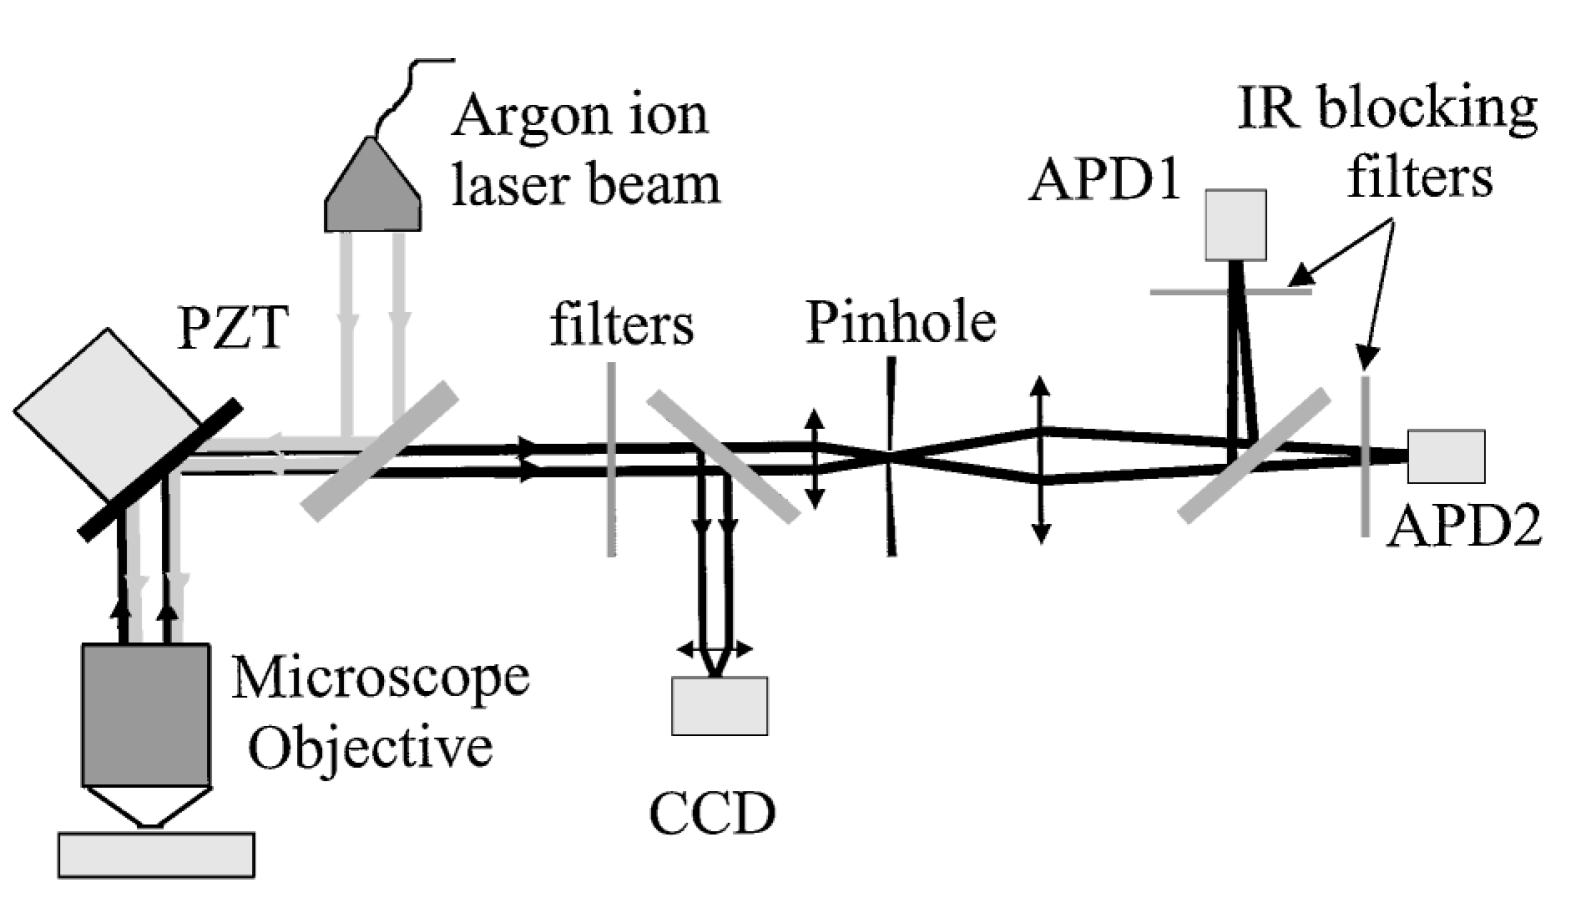
\includegraphics[scale=0.6]{Versuchsaufbau.PNG}
\caption{Schematischer Versuchsaufbau eines Hanbury Brown-Twiss-Setup zur Messung der Korrelation von Photonen von NV-Zentren. \cite{brouri}  }
\label{fig:Versuchsaufbau}
\end{figure}
Als erstes wird die y-Richtung festgehalten um den richigen Werte f\"uer die z-Richtung zu erhalten. 
Danach kann die z-Richtung festgehalten werden und die x-y-Ebene gemessen werden. 
F\"ur die Messung muss nun ein Bereich ausgew\"ahlt werden, in dem es  ein NV-Zentrum gibt.  
Dieser Bereich sollte in dem Histogramm f\"ur die x-y-Ebene eine engef\"ahr runde Form habe. 
Au{\ss}erdem darf der Bereich nicht zu gro{\ss} sein und es d\"urfen auch nicht zuviele Photonen aus diesem Bereich emitiert werden. 
Diese Kriterien sind notwendig, da eine Emission von Photonen in Diamaten auch andere Ursachen, zum Beispiel Fehlstellen, haben kann. 
Nach dem ein Breich f\"uer die Messung ausgew\"ahlt worden ist, muss der Autofokus aktiviert werden, damit ein Abdriften der gew\"unschten Stelle vermieden werden kann. Gemessen wird nun f\"ur dieses NV-Zentrum, die Zeitdifferenzen zwischen dem Eintreffen der Photonen an den beiden Photodioden. 
Diese Messung soll f\"ur zwei NV-Zentren durchgef\"uhrt werden. 
Um ausagekr\"aftige Resultatte zu erziehlen, soll jede Messung ungef\"ahr zwei Stunden lang dauern. 
Als drittes soll ein Gebiet des Diamanten gemessen werden, bei dem es sich nicht um ein NV-Zentrum handelt. 
Dazu soll ein Bereich ausgew\"ahlt werden, in dem ein Vielfaches der Photonen eines NV-Zentrums emittiert wird. Aufgrund der stärkeren Emission reicht eine viel kleinere Messdauer aus. 

%TO DO: bild aus paper einfuegen, mit quellenangabe


\section{Analysis}


\section{Zusammenfassung}
In diesem Versuch sind die magnetischen Eigenschaften einer magnetooptischen Disk untersucht worden. Gemessen wurden Hysteresekurven für unterschiedliche Temperaturen. Die gemessene Kurven wurde um ihren Offset und den Einfluss der schützenden Polymerschicht korrigiert. Aus den gemessenen Daten ist die Koerzitivfeldstärke ermittelt worden, mit der die Kompensationstemperatur 
\begin{equation}
T_\mathrm{comp}  = 279.45 \pm 2.73\ \mathrm{K} 
\end{equation}
berechnet werden konnte.
Der Kerr-Winkel nimmt bei steigenden Temperaturen leicht ab.
Er bleibt dabei in einem Bereich von \SI{0.7}{\degree} bis \SI{0.95}{\degree}.

\section{Appendix}
You will find the tables with the original measurement data in the following.

\begin{table}[htbp]
\centering
\caption{
    Measurements for $\Psi^{+}$.
    The angles $\alpha$ and $\beta$ are the angles at the two polarizers.
    The coincidence count rates $C(\alpha,\beta)$ are taken five times as average over \SI{10}{\second} in order to reduce noise.
}
\label{tab:mesplus}
\bigtableplus
\end{table}

\begin{table}[htbp]
\centering
\caption{
    Measurements for $\Psi^{-}$.
    The angles $\alpha$ and $\beta$ are the angles at the two polarizers.
    The coincidence count rates $C(\alpha,\beta)$ are taken five times as average over \SI{10}{\second} in order to reduce noise.
}
\label{tab:mesminus}
\bigtableminus
\end{table}

\begin{table}[htbp]
\centering
\caption{
    Measurements for the tomography.
    The states S1 and S2 of photon 1 and 2 are choosen to provide the calculation of the density matrix of the light.
    The angles of the polarizers P1 and P2 and the $\lambda/4$ plates L1 and L2 for photon 1 and 2 must be choosen as mentioned.
    The coincidence count rates $C(\alpha,\beta)$ are taken five times as average over \SI{10}{\second} in order to reduce noise.
}
\label{tab:mestom}
\bigtabletom
\end{table}
\printbibliography

\end{document}
